\chapter{Referêncial Teórico} \label{RevisaoBibliografica}

Este capítulo tem como objetivo apresentar uma contextualização sobre os temas da pesquisa, utilizada como base teórica para o desenvolvimento do trabalho. Para apresentar da melhor forma o estudo serão analisados artigos e trabalhos sobre a plataforma arduino, sobre sensores compatíveis com a tecnologia, e sobre o conceito de Internet das coisas. Além disso, será estudada a estrutura meteorológica brasileira para o contexto aeronáutico, bem como uma visão geral da plataforma ThingSpeak.

\section{Fundamentação Teórica}

\subsection{Plataforma Arduino}

Conforme as ideias de \cite{mcrobertssao}, o arduino é uma plataforma embarcada, composta por hardware e software de código aberto, desse modo, facilita a criação de inúmeros projetos independentes interativos, de automação, monitoramento. A ferramenta integrada de desenvolvimento(IDE), baseada na linguagem de programação C. 

Segundo \cite{banzi2011primeiros} a Vantagem de se utilizar Arduino pode ser resumida em:
\begin{itemize} 
    \item É um ambiente multiplataforma; o código para os dispositivos podem ser criado e executado no Windows, Macintosh e Linux. Além possui IDE compatível com todos os ambientes.
    \item Não é necessária uma porta serial nem adaptadores para o carregamento do código que é carregado por um cabo USB.
    \item  O hardware e software são de fonte aberta sendo possível fazer o download do diagrama de circuito, comprar todos os componentes e criar seu modelo próprio, sem ter de pagar direitos autorais aos criadores originais.
    \item O hardware é barato em caso de avaria pode não representar em grandes prejuízos e fácil substituição.
    \item Tem uma comunidade muito ativa o que facilita no esclarecimento de dúvidas e problemas.
\end{itemize}

O maior benefício para o crescimento da plataforma é sem dúvidas a força da comunidade, pois, em muitas plataformas que não possuem membros ativos e a única informação são os manuais dos fabricantes que são insuficientes para todas as situações. 

\subsubsection{Arduino UNO}
    
A figura \ref{fig:arduino} representa os principais componentes da placa arduino UNO.

\begin{figure}[!ht]
    \centering
    \caption{Componentes do Arduíno UNO}
    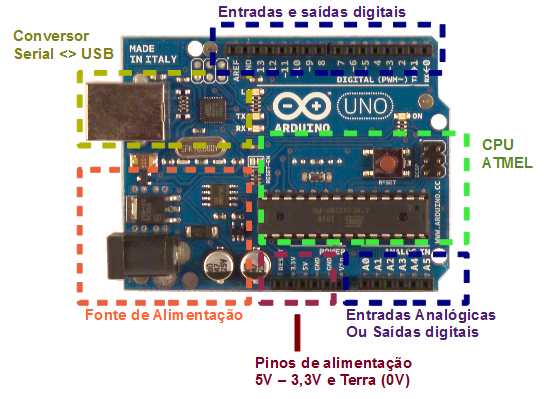
\includegraphics[scale = 0.75]{Figuras/Fig1_arduino.png}
    \legend{Fonte:  https://wiki.sj.ifsc.edu.br/index.php/MCO018703\_2018\_1\_AULA08}
    \label{fig:arduino}
\end{figure}

\textbf{Fonte de Alimentação}:Tem o principal papel de receber energia de alimentação externa, que pode variar entre as tensões entre 7 a 20 Volts com uma corrente elétrica mínima de 300mA. Existem adaptadores que ligam a fonte a uma pilha de 9V ou diretamente na tomada.

\textbf{Plugn USB e Conversor Serial/USB}: Tem como responsabilidade carregar o código da IDE do Arduíno para a placa. Pode ser utilizada como fonte de alimentação energética.

\textbf{Unidade Central de Processamento ATMEL}: É o circuito integrado responsável por executar o código enviado a placa. Cada placa tem  diferentes tipos de microcontroladores, memórias internas e capacidade de processamento. Normalmente são chips da marca ATMEGA

\textbf{Pinos de Alimentação}: Regulam tensões mínimas e máximas da voltagem provenientes de fontes externas ou da alimentação USB. As tensões possíveis dos pinos de alimentação são: 3,3V, 5V e 0V(GND).

textbf{Entradas e Saídas Digitias}: São portas lógicas usadas para enviar ou receber sinais digitais para sensores, ou dispositivos conectados a placa com a informação de 0V(desligado) a 5V(ligado).

\textbf{Entradas Analógicas}: São portas que tem o papel de realizar leituras de sinais analógicos de sensores ligados a placa como luz, movimento, temperatura, entre outros.

Inicialmente para o trabalho foi cogitado utilizar a placa NODEMCU, pois, o número de portas lógicas digitais e analógicas eram suficientes para o projeto com a facilidade da conexão de Internet sem fio do módulo ESP8266-12E seria útil na transmissão de dados. Entretanto, o sensor de biruta eletrônica que é analógico não produziu resultados satisfatórios de mensuração. O comportamento para a falha foi devido ao nível de tensão que a placa utiliza na porta analógica A0, a única do NODEMCU possui uma tensão de 1V. O sensor analógico de biruta eletrônica, segundo o fabricante, é adequado para tensões de 5V e internamente é equipado com resistores que variam de 10K$\Omega$ até 80K$\Omega$ com a função de reduzir a voltagem de entrada resultando em uma voltagem de saída mais baixa. Para um nível de tensão de entrada de 1V em resistências dessa grandeza o resultado não seria preciso, por que além da incompatibilidade existe a varição de voltagem do equipamento que é de aproximadamente $\pm$ 0.2V.

Por esse motivo no trabalho foi utilizado uma placa Arduino UNO pois ela suportou bem todos os sensores utilizados no trabalho.


\subsection{Internet das Coisas}

A iot já está mudando a maneira como pessoas e objetos se relacionam entre si\cite{zmud2018primer}. Imagine uma geladeira capaz de informar para o smartphone que a quantidade de ovos em seu interior está abaixo do suficiente para fazer um bolo. Então um aplicativo do smartphone com essa informação enviada pela geladeira já faz uma rota de possíveis locais que vendem ovos e manda uma notificação para o usuário cada vez que ele se aproxima de um local de compra. 

Não basta o objeto estar conectado à Internet que já é sinônimo de iot, mas além de processar dados ele pode tomar pequenas decisões de forma inteligente para que haja intervenção humana. Por exemplo, se a temperatura atingir 40°C, em uma sala técnica de informática, será enviado uma notificação para que o responsável possa tomar alguma ação. 

Uma boa síntese da variedade de questões foi feita por \cite{atzori2010internet}. A figura \ref{fig:IoTParadigma} é uma tentativa de resumir as principais áreas de pesquisa e tipos de aplicação e oferecer uma visão mais completa da IOT, que segundo o autor da imagem é melhor entendida como um paradigma computacional formado pela sobreposição de visões orientadas às coisas, à Internet e à semântica.
A visão de Atzori é muito voltada para a tecnologia, não vê as finalidades nos quais o usuário pode se deter como usabilidade, autorização e autenticação para o acesso à informação.
\\
\\
\\
\\
\\
\\
\\
\\
\begin{figure} [!h]
    \centering
    \caption{O paradigma da Internet das Coisas}
    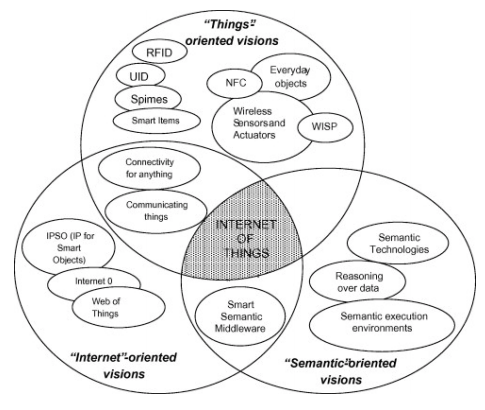
\includegraphics[scale = 0.7]{Figuras/Internet_das_Coisas.png}
    \legend{Fonte: (ATZORI, 2010, p. 2)}
    \label{fig:IoTParadigma}
\end{figure}


Outra abordagem mais simples do conceito de iot é dividi-lo em três camadas. Segundo \cite{zmud2018primer} a primeira representada por sensores com a responsabilidade de capturar dados. Que transmite esses dados para a segunda camada de comunicação responsável por filtrar, agregar informações e a última camada representada pela nuvem como a responsabilidade de manter, analisar e gerar ferramentas de visualização de conhecimento para definir ações futuras.

\begin{figure} [!h]
    \centering
    \caption{Internet das Coisas em 3 Camadas}
    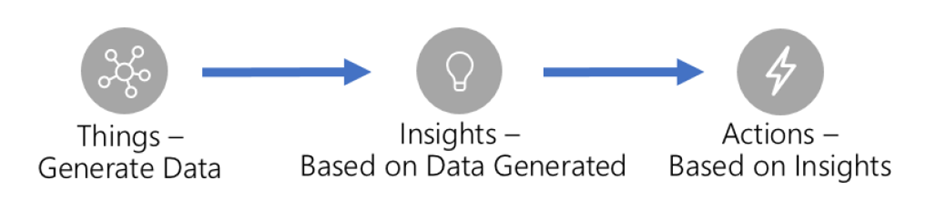
\includegraphics [scale = 0.40] {Figuras/framework_IOT.png}
    \legend{Fonte: Microsoft Azure IOT Framework}
    \label{fig:4}
\end{figure}

Um fator que permeia muitas pesquisas na área de Internet das coisas é a segurança, que é um elemento que deve envolver todas as camadas. Colaborando com estratégias para caso um componente for comprometido não faça prejuízo à estrutura. Para esse fim são utilizadas tecnologias como criptografia, controle de acesso com autorização e autenticação, identificação dos dispositivos entre outras medidas para garantir a integridade do sistema.

No que se refere às aplicações, podemos notar a presença de iot no nosso cotidiano. Como, por exemplo, sensores que detectam a presença física em uma determinada área e enviam informações para uma central de controle. Com isso é possível criar aplicação para controle de acesso de pessoas, dispositivos inteligentes podem se mover para a área que deve ser controlada por um determinado período no caso de aeroportos onde é necessário quando existe demanda\cite{hui2008rfid}.

Também já existem plataformas industriais para Internet das Coisas como é o caso de empresas como a Amazon com a AWS iot e Amazon Alexa, Microsoft como Azure IOT e IBM com a IBM Watson iot.


\subsection {Estrutura Meteorológicas Brasileira para o Contexto Aeronáutico}

Um fator que contribuiu para o início do desenvolvimento da meteorologia brasileira foi um naufrágio, na costa do Rio Grande do Sul motivado por um temporal em 11 de julho de 1887 \cite{barboza2006historia}. Na época o Brasil não tinha serviço de previsão do tempo. A tragédia motivou alguns cientistas a tentar explicar o que aconteceu, porém, como os dados da época eram escassos e o conhecimento da dinâmica atmosférica também não tiveram sucesso.

Vinte anos depois da ocorrência, cientistas brasileiros adquiriram conhecimento para elaboração de mapas sinóticos desde modo foi possível explicar o que aconteceu em 11 de julho de 1887 e também iniciar o serviço de previsão do tempo no Brasil\cite{oliveira2009inmet}.

\begin{figure} [!ht]
    \centering
    \caption{Exemplo de mapa sinótico}
    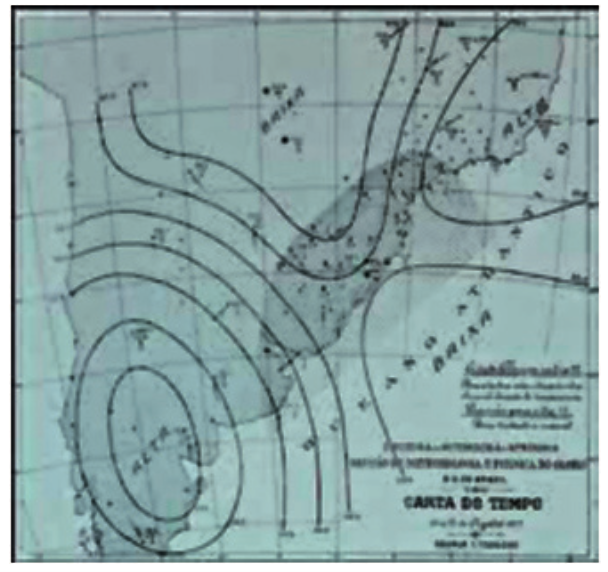
\includegraphics [scale = 0.35] {Figuras/mapa_sinotico.png}
    \legend {Fonte: (Oliveira,2009 p.36)}
    \label{fig:4}
\end{figure}

A meteorologia no Brasil foi se aprimorando com técnicas vindas do exterior e qualificação de profissionais e se chegou até a seguinte estrutura:

\begin{itemize}
    \item Instituto Nacional de Meteorologia (INMET) do Ministério da Agricultura
    \item Centro de Previsão do Tempo e Estudos Climáticos do Ministério da Ciência e Tecnologia(CPTEC)
    \item Meteorologia Aeronáutica do Comando da Aeronáutica e Meteorologia Marítima do Comando da Marinha, ambas pertencentes ao Ministério da Defesa e às Meteorologias Estaduais: FUNCEME(Ceará), SIMEPAR(Paraná), EPAGRI/CIRAM(Santa Catarina) entre outros.
\end{itemize}

O órgão oficial de meteorologia brasileiro é o INMET \cite{oliveira2009inmet}. É o representante do país junto à organização Meteorológica Mundial(OMM), criada em 1950 é o organismo responsável das Nações Unidas pela meteorologia, no que diz respeito ao clima, tempo e ciências afins.

No contexto aeronáutico, o serviço de meteorologia é regulamenta pela Organização da Aviação Civil Mundial(OACI), sendo o DECEA, o órgão normatizador e fiscalizador, conforme os padrões de OMM, OACI e os interesses nacionais. O serviço tem como finalidade a observação da atmosfera, visando eficiência e a segurança das atividades aéreas.

A segurança das atividades aéreas usando informações meteorológicas, a grosso modo, é basicamente informar ao piloto as condições do tempo que possam ser encontradas desde do momento da decolagem até o momento do pouso. Condições que são observadas, em parte, e prognosticadas no todo destacando as adversidades para o voo como: áreas de turbulências, aéreas de formações de gelo, trecho de visibilidade reduzida, teto baixo. 

Segundo \cite{costa2008meteorologia} o planejamento do voo começa com a observação e análise das condições do tempo. Condições que são observadas somente nas proximidades dos aeródromos, num raio de 20 km enquanto a previsão cobre toda a rota utilizada por um voo.

Para que a informação cumpra seu papel existe diferentes setores na meteorologia aeronáutica conforme exposto por \cite{henrique2005meteorologia}:
\begin{itemize}
    \item Rede de Estações Meteorológicas(REM).
    \item Estação de Radares Meteorológicos(ERM).
    \item Bancos de Dados Meteorológicos.
    \item Sistema de divulgação de informes meteorológicos
\end{itemize}
    
A rede de estações meteorológicas é formada por estações de superfície e de altitude(EMA). E divulgação de informações operacionais é feita por meio oficial através da REDEMET \cite{redemet2020homepage} que é uma plataforma mantida pela FAB que tem como objetivo a integração dos serviços de meteorológica com o acesso a informações de modo rápido e eficiente.


\subsection{Estação Meteorológica de Superfícies}

Segundo a instrução do comando da aeronáutica(ICA) \cite{BRASILMCA104}, as estações meteorológicas têm a responsabilidade de coletar, processar e registrar dados meteorológicos de superfície e altitude para apoio à navegação aérea. Podendo ser de três tipos:
\begin{itemize}
    \item Estações Meteorológicas de Altitude (EMA)
    \begin{citacao}
As Estações Meteorológicas de Altitude têm por finalidade coletar, através de Radiossondagem, dados de pressão, temperatura, umidade, direção e velocidade do vento, nos diversos níveis da atmosfera. 
    \end{citacao}
    \item Estações Meteorológicas de Superfície (EMS)
    \begin{citacao}
As Estações Meteorológicas de Superfície têm por finalidade efetuar a coleta e o processamento de dados meteorológicos à superfície para fins aeronáuticos e sinóticos. Devem ser instaladas nos aeródromos e fazem parte da rede básica da Organização Meteorológica Mundial (OMM), quando equipadas apropriadamente.
\end{citacao}

\end{itemize}

Conforme exposto somente as EMS são instaladas nos aeródromos e elas são classificadas em três categorias conforme \cite{BRASILMCA104} EMS-1, EMS-2, EMS-3. A principal diferença entre está nos dispositivos que compõem cada categoria da estação. Para expor de modo claro a diferença de cada categoria de estação por sensores é interessante explicar o papel de cada sensor conforme \cite{DECEA}

\begin{itemize}
    \item Anemômetro: fornece a direção e velocidade (média e máxima) do vento nas zonas de ponto de toque das pistas; 
    \item Transmissômetro: fornece os valores de Alcance Visual na Pista ao longo das pistas;
    \item Tetômetro: fornece a altura da base das nuvens, referente ao sítio do marcador médio. Na impossibilidade de instalação no marcador médio, o tetômetro poderá ser instalado junto ao sítio meteorológico da cabeceira principal ou próximo ao sítio do marcador interno; 
    \item sensores de temperatura do ar e de umidade relativa: fornecem a temperatura do ar e a umidade relativa, referentes ao sítio meteorológico principal;
    \item barômetro: fornece a pressão atmosférica, informando valores de Pressão reduzida ao nível do mar pelo gradiente vertical da atmosfera padrão(QNH),Pressão real ao nível do mar(QFF) e a Pressão atmosférica ao nível de elevação do aeródromo ou na cabeceira da pista)(QFE), localizado no sítio meteorológico principal; 
    \item pluviômetro: fornece a quantidade de precipitação, referente ao sítio meteorológico principal;
\end{itemize}

A EMS-1 e a categoria de estação mais completa ela possui todos os sensores listado acima. A EMS-2 possui todos os sensores listados acima exceto o transmissômetro. Já a EMS-3 a categoria mais simples possui os sensores.
\begin{itemize}
    \item Anemômetro: para informar o vento do aeródromo não necessariamente o das zonas de ponto de toque da pista.
    \item Os sensores de temperatura e de umidade relativa do ar e barômetro: também referente ao aeródromo não ao local meteorológico principal.
\end{itemize}

Além dos tipos de equipamento o \cite{DECEA} define como deve ser feita as observações meteorológicas podendo ser feitas de forma regular, especial ou local.

A observação regular é realizada em horários pré-fixados, em intervalos de uma hora e deve ser confeccionada e divulgada no formato de METAR que são mensagens meteorológicas para uso Operacional.

A observação especial quando ocorre variações meteorológicas consideráveis como, por exemplo: quando a velocidade média do vento à superfície mudar em 10 kt ou mais, em relação à última observação. Quando existir fenômeno ou combinação deles como nevoeiro, tempestade de poeira, precipitação congelante, trovoadas, nuvens do tipo funil entre outros. A observação especial deve ser divulgada em formato SPECI conforme documentações.

A observação local é aquela realizada quando ocorrer um acidente ou incidente aeronáutico no aeródromo, ou em sua vizinhança. Posteriormente, poderá ser fonte de informações para eventual investigação. Ela tem início no momento que o acidente ou incidente ocorre. 

Este trabalho utilizará das observações regulares no formato METAR para testar se os dados coletados pelo protótipo elaborado no trabalho podem ser consideradas iguais aos da plataforma REDEMET.

\subsection{Sensores}

Na eletrônica um sensor é um dispositivo com qualquer componente elétrico ou circuito eletrônico que permite a análise de uma determinada condição do ambiente\cite{neto2020eletronica}. Podendo ser
divididos em dois tipos: analógicos e digitais. Essa divisão é feita pelo modo como o dispositivo responde à variação de uma determinada condição.

Os sensores analógicos têm como base o sinal analógico. São sinais que, mesmo com a limitação entre dois valores de tensão, eles podem assumir infinitas representações intermediárias. Para cada nível da condição medida haverá um sinal de tensão correspondente. Como exemplo posso destacar, um sensor de luminosidade, que é um dispositivo cuja resistência varia de acordo com a quantidade de luz, quanto mais intensa à iluminação verifica-se que a resistência reduz de forma gradual.

\begin{figure} [h!]
    \centering
    \caption{Exemplo de sensor analógico}
    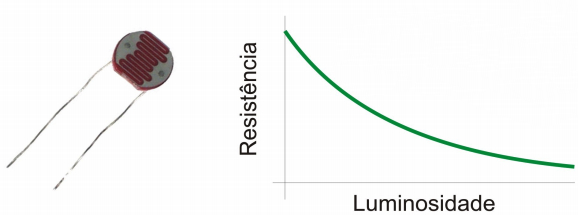
\includegraphics [scale = 0.5] {Figuras/sensor_analogico.jpg}
    \legend{Fonte: Adaptada.   encurtador.com.br/fI127}
    \label{fig:cinco}
\end{figure}


Os sensores digitais têm como base, níveis de tensão bem definidos. Eles podem ser descritos como Alto ou Baixo, Verdadeiro ou Falso, "1" ou "0". Eles usam da lógica binária, que é o alicerce do funcionamento dos sistemas digitais. Esse tipo de sensor alterna entre estados bem definidos. Como exemplo podemos descrever um sensor de infravermelho Conforme figura \ref{fig:infraVermelho}. Se o feixe de infravermelho atinge o receptor, teremos um nível de tensão baixo. Quando algo bloqueia o caminho da luz infravermelha pode se considerar nível de tensão alto.

\begin{figure} [h!]
    \centering
    \caption{Exemplo de senor digital}
    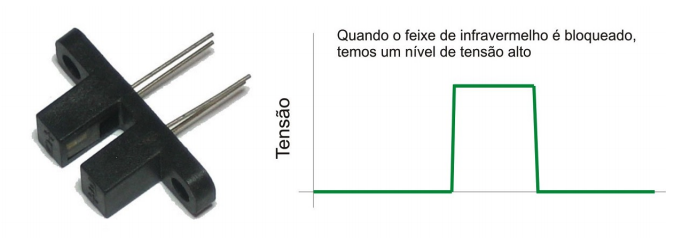
\includegraphics [scale = 0.5] {Figuras/sensor_digital.png}
    \legend{Fonte:  https://bityli.com/OGb1E }
    \label{fig:infraVermelho}
\end{figure}

O fato é que em projetos que envolve sensores sempre iremos encontrar os dois tipos. Na plataforma arduino utilizamos as portas lógicas digitais isso fornece a capacidade de receber e enviar sinais digitais e quando se utiliza portas analógicas é possível capturar sinais analógicos e mapeá-los para sinais digitais.

\subsubsection {Anemômetro}

O anemômetro utilizado no trabalho e do tipo concha que é composto por três ou mais conchas de formato especial montada simetricamente formando ângulos de 90 graus com um eixo vertical. A velocidade do vento, independentemente de direção, faz mover o conjunto das conchas um mecanismo que conta as rotações e então a velocidade é calculada com o auxílio de um dispositivo de contagem no caso do modelo escolhido para esse trabalho utiliza um sensor Reed Switch \cite{USINAINFOBLOG}.

\begin{figure} [!h]
    \centering
    \caption{Anemômetro tipo concha - Modelo SV10}
    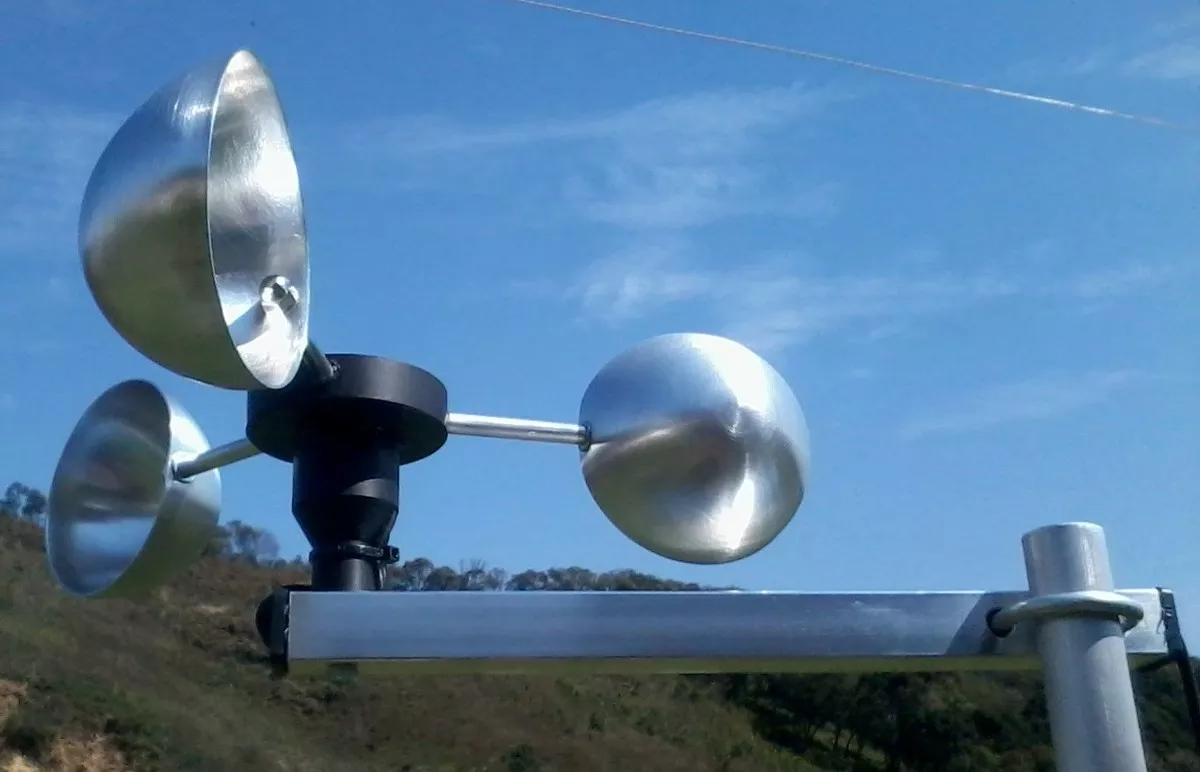
\includegraphics[scale=0.25]{Figuras/ane_SV10.png}
    \legend{Fonte: Adaptada https://www.usinainfo.com.br/blog/ }
    \label{fig:anemometro}
\end{figure}

O modelo de anemômetro SV10 foi escolhido para o trabalho por que foi o único encontrado no mercado. Segundo o manual do fabricante \ref{manAnemot} ele trabalha com várias tensões 3V3, 5V e 12V, e formado por três conchas feitas de alumínio, segundo a descrição do equipamento ele pode medir ventos de até 120 Km/h\cite{USINAINFOBLOG}.

\subsubsection{Biruta}

Birutas eletrônicas que usam a energia elétrica para medir a direção do vento. O modelo escolhido para o trabalho DV10 por que foi o único encontrado no mercado. Ele Consegue medir a direção do vento nos pontos cardeais e colaterais, ou seja, nos graus (0º, 45º, 90º, 135º, 180º, 225º, 270º e 315º). Esse equipamento recebe uma voltagem de entrada de 5V e conforme a direção do vento a aplicado o conceito de divisão de tensão com resistores variando de 10K$\Omega$ até 80k$\Omega$ gerando uma voltagem final conforme anexo \ref{manAnemog} correspondente a direção do vento.

\begin{figure} [!h]
    \centering
    \caption{Biruta Modelo DV10}
    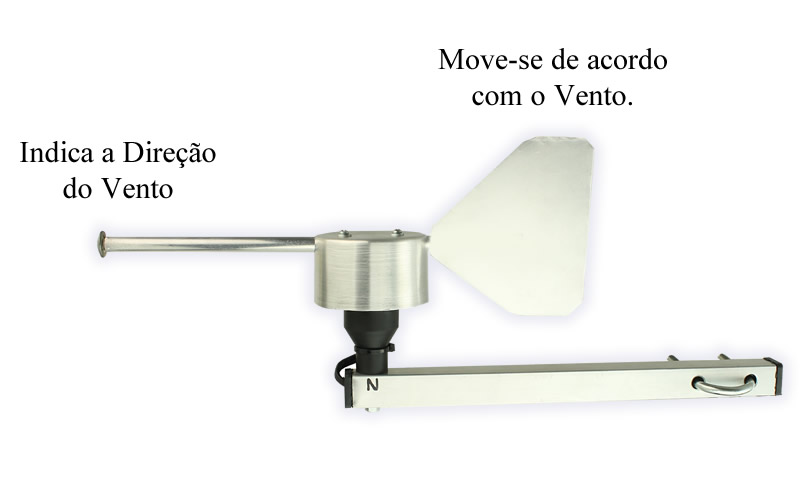
\includegraphics[scale=0.25]{Figuras/posicao-da-pa-e-indicacao.jpg}
    \legend{Fonte: Adaptada https://www.usinainfo.com.br/ }
    \label{fig:biruta}
\end{figure}


\subsubsection{Sensor de Temperatura}

Para sensor de temperatura foram encontrados vários modelos no mercado. Para decidir qual sensor deverá fazer parte da estação foi utilizado o trabalho de \cite{konstantinoscomparative} que compara três sensores para medir temperatura do mercado são MCP9808, BMP180 e o DHT22 com as medições feitas em um termômetro de mercúrio.

O sensor que teve uma maior aproximação com as medições feitas no termômetro de mércurio foi o BMP180 com uma taxa de erro medida através do uso de regressão linear. No mercado o sucessor do BMP180 é o sensor BMP280 que tem a mesma finalidade, porém, com um consumo energético mais eficiente e precisões melhores e tamanho reduzido. Na tabela 2.1 podemos notar as principais diferenças entre os modelos.

\begin{table}[!h]
\centering
\begin{tabular}{|l|c|c|}
\hline
\textbf{Parâmetro}                           & \textbf{BMP180} & \textbf{BMP280} \\ \hline
Dimensões                                    & 3,6 mm x 3,8mm  & 2,0 mm x 2,5 mm \\ \hline
Tensão Mínima                                & 1,6V            & 1,2V            \\ \hline
Consumo de Corrente Elétrica Médio           & 12$\mu$A         & 2,7$\mu$A        \\ \hline
Precisão para medição de pressão atmosférica & 1Pa             & 0.016Pa         \\ \hline
Precisão para medição de temperatura         & 0,1 ºC          & 0,01 ºC         \\ \hline
\end{tabular}
\caption{Diferenças entre os sensores BMP180 e BMP280}
\label{tab:tablebmp}
\end{table}

O sensor de temperatura escolhido para formar a estação do trabalho será o BMP280 conforme visto na tabela \ref{tab:tablebmp} ele tem alta precisão e baixo consumo energético.

\subsubsection{Sensor de Pressão Atmosférica}

O sensor BMP280 além de medir temperatura ele também mede pressão atmosférica com a finalidade de reduzir custos também foi escolhido para a mensuração dessa variável conforme visto na tabela\ref{tab:tablebmp} ele pode mensurar uma faixa entre 940 e 1100 hPa. Tem uma precisão de $\pm$0,016Pa.

\begin{figure} [!h]
    \centering
    \caption{Sensor BMP280}
    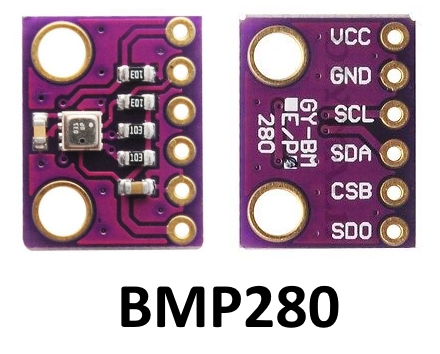
\includegraphics[scale=0.5]{Figuras/BMP280_Pinout.jpg}
    \legend{Fonte: https://forum.arduino.cc/index.php?topic=654763.0}
    \label{fig:bmp280}
\end{figure}

\subsubsection{Sensor de Umidade Relativa do Ar}

Na plataforma arduino os sensores de umidade relativa do ar mais encontrado no mercado são o DHT11 e DHT22. Os dois modelos são da mesma fabricante. A diferença entre ambos conforme \cite{AutoCoreBlog} pode ser entendida na figura abaixo:

\begin{table}[!h]
\centering
\begin{tabular}{|l|c|c|}
\hline
\textbf{Parâmetro}           & \textbf{DHT 11} & \textbf{DHT 22} \\ \hline
Tensão de Alimentação        & 3V - 5.5V       & 3.3V - 6V       \\ \hline
Corrente Máxima              & 2.5mA           & 1.5mA           \\ \hline
Faixa de Leitura Umidade     & 20 - 80\%       & 0 - 100\%       \\ \hline
Precisão Umidade             & 5\%             & 2\%             \\ \hline
Faixa de Leitura Temperatura & 0 até 50 ºC     & -40 até 125 ºC  \\ \hline
Precisão Temperatura         & 2 ºC            & 0,5 ºC          \\ \hline
Intervalo de Medições        & 1s              & 2s              \\ \hline
\end{tabular}
\caption{Diferenças entre DH11 e DHT22}
\label{tab:dhtsensor}
\end{table}

Fica bem exposto na tabela \ref{tab:dhtsensor}, que o DHT11 ele é duas vezes mais rápido que o DHT22 em suas medições. Sua precisão em relação a umidade relativa do ar não é boa podendo chegar a $\pm$ 5\% além de consumir mais energia comparado ao DHT22. No trabalho de \cite{ribeiro2016avaliaccao} e demonstrado que realmente a faixa de erro de 2\% se comprova. Vale notar que os dois podem ser alimentados com a faixa de tensão entre 3.3V a 5.5V. Em relação a custo também o DHT11 é bem mais barato que o DHT22. O DHT11 custa em média 70\% que DHT22.

Nesse trabalho se foi escolhido o sensor de DHT22 por ser muito utilizado no mercado e também pelo baixo consumo energético com a faixa de precisão para umidade com menor percentual de erro.

\subsection{Plataforma ThingSpeak}

ThingSpeak é uma plataforma para Internet das coisas que permite a agregação, a visualização de dados em tempo real na nuvem. Possibilitando o envio e leitura de dados por dispositivos, criando visualizações gráficas em tempo real. A plataforma permite o envio de alerta quando determinadas condições são atingidas para redes sociais como Twitter e Twilio. Além disso, dentro do ambiente da plataforma é possível a execução de código da linguagem MATLAB que é usada para pre-processamento, visualização e analise \cite{ThinkSpeak}. A grande vantagem de se usar o Thingspeak e a facilidade para configuração de um servidor sem a necessidade de desenvolvimento de um sistema completo para WEB.

A plataforma Thingspeak também permite o armazenamento dos dados coletados e a disponibilização dos dados em formato de XML ou JSON e também permite a leitura dos dados através de uma requisição HTTP. Os dados coletados são armazenados em canais que permitem o armazenamento de até oito tipos de dados diferentes. Além de informações de descrição, altitude, latitude e longitude. Assim que um canal é criado ele tem uma sequência de números únicos um ID. Os dados podem ser acessados através da API do Thingspeak que necessita de uma chave de acesso gerada pela própria plataforma para as operações de leitura e operações de escrita de dados. Os canais eles pode ter visualizações públicas ou privadas. Quando o canal é público não é necessário utilizar chave de leitura para o acesso.

\begin{figure}[h!]
    \centering
    \caption{Plataforma Thingspeak}
    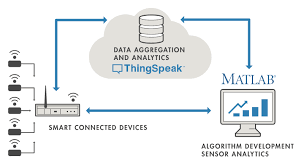
\includegraphics{Figuras/think_speak.png}
    \legend{Fonte: https://thingspeak.com/ }
    \label{fig:thinkSpeak}
\end{figure}

Existem outras plataformas de IOT concorrentes do Thingspeak destaco a plataforma Blynk que foi considerada para uso no projeto. Ela possui com três componentes um aplicativo, um servidor e a placa. Tem a vantagem de possuir configurações como a de conexão com a Internet para placas mais utilizadas no mercado como arduino UNO, NODEMCU, ESP8266. Permitindo também essa comunicação por portas seriais com uma estação de trabalho \cite{8473224}. O Blynk é parte gratuito para uso de bibliotecas, servidor e hospedagem na nuvem. A forma de monetizar está no aplicativo esse serviço tem uma série de widgets para visualização de informações ou botões para acionar comandos. Cada widget consome uma moeda virtual da plataforma ao iniciar uma conta o usuário recebe um valor inicial e vai gastando conforme as escolhas de componentes na plataforma.

\begin{figure}[h!]
    \centering
    \caption{Widgets da Plataforma Blynk}
    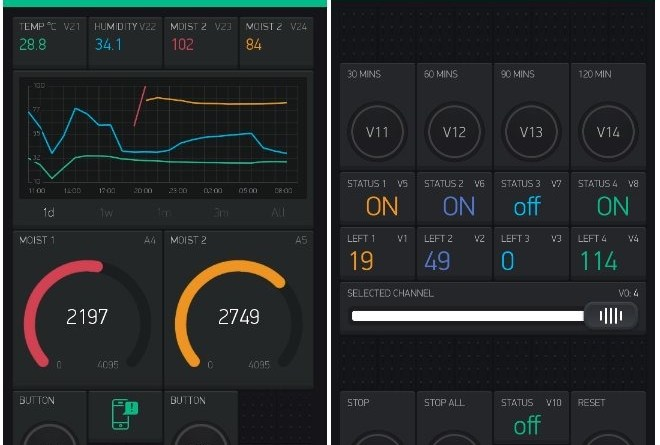
\includegraphics[scale=0.5]{Figuras/blynk_app.jpg}
    \legend{Fonte: https://blynk.io/ }
    \label{fig:blynk}
\end{figure}

A grande desvantagem dessa plataforma é que a visualização das informações fica dependente apenas dos widgets oferecidos pelo serviço, apesar de possuir uma grande variedade de componentes, O código do aplicativo é fechado então não é possível modificar essas visualizações conforme necessidade. Outro aspecto negativo é que se os componentes não forem bem posicionados pode gerar confusão na interpretação da informação que é vista apenas por dispositivos móveis o que limitaria no caso de uma necessidade de expor em uma televisão ou painel de informações não seria adequado.

O Thingspeak tem suporte a linguagens de programação como Ruby, Python e Node.js. Linguagens bem populares no meio WEB e a facilidade de integração com Python permite o acesso a várias bibliotecas que o Python possui para trabalhar com análise de dados não obrigando o desenvolvedor a utilizar a linguagem que já vem com a plataforma o MATLAB.

O serviço do Thingspeak tem também suas limitações como a operação de atualização só pode ser feita a cada 15 segundos. A razão para a limitação e que muitas atualizações podem sobrecarregar a plataforma. Outra desvantagem é o número limitado de gráficos apesar de outros serviços nem possuir essa característica de plotar informações. Também não existem informações de onde estão armazenados os dados nem dos mecanismos de segurança assim como não é informado por quanto tempo os dados ficarão armazenados nos servidores.

\subsection{Protocolo MQTT}

O MQTT segundo \cite{torres2016analise} é um protocolo próprio para comunicação entre máquinas(M2M) opera com o TCP/IP e funciona bem com redes de alta latência, com instabilidade na comunicação e baixa largura de banda.

Conforme descrito em \cite{de2017internet} O MQTT funciona através de três estruturas:

\begin{itemize}
\item MQTT Broker: É o servidor onde os dados ficam disponíveis para eventuais dispositivos assinantes no caso desse projeto será a plataforma ThingSpeak.
\item Publisher MQTT: É o dispositivo que gera a informação e publica no servidor. No caso desse trabalho dividimos a responsabilidade de publicar em um script em Python e gera os dados que será feito através do código embarcado no arduino.
\item Subscriber MQTT: São os dispositivos interessados nos dados do serviço no caso em análise será o aplicativo disponibilizado para visualização na plataforma Thinspeak.
\end{itemize}

As vantagens de utilização do protocolo é na baixa necessidade de processamento para o envio de mensagens e no baixo consumo de banda com seu cabeçalho muito pequeno cerca de 2 bytes segundo \cite{mota2017analise}. A desvantagem é que o protocolo não possui uma camada de segurança então utiliza os mecanismos do TCP/IP.


\section{Trabalhos Relacionados}

Nessa seção apresento projetos que já desenvolveram estações meteorológicas utilizando a plataforma arduino. Foram escolhidos trabalhos dos últimos cinco anos que utilizaram conceitos similares para o desenvolvimento de um protótipo. Primeiramente será feito um comentário sobre cada trabalho e por fim será apresentada uma tabela \ref{tab:comp_trabalhos} com as principais características dos trabalhos.

No trabalho de \cite{torres2015aquisiccao} o autor propõe a criação de uma estação meteorológica simplificada com a utilização da plataforma arduino com objetivo de reduzir custos das estações meteorológicas disponíveis no mercado. O trabalho conta com a utilização de três sensores: temperatura, luminosidade e umidade do ar. São realizados testes em laboratório para comparar dados de uma estação, do Instituto Nacional de Meteorologia(INMET), mais próxima geograficamente do local do trabalho. Os resultados são apresentados graficamente baseados na interpretação do autor, não há a presença do conceito de iot que poderia facilitar a disponibilização da informação e redução de custos. Nesse projeto todos os dados coletados foram mantidos em um módulo de cartão de memória.

Na elaboração de estação meteorológica feita por \cite{da2016estaccao} podemos encontrar a utilização de sensores para: temperatura, precipitação atmosférica, intensidade da luz solar, umidade do ar, pressão atmosférica, velocidade do vento. O autor também adquiriu um módulo à parte para conexão com a Internet, o modulo ESP8266, e criou um sistema WEB próprio para receber os dados dos sensores. O autor comparou os custos dos sensores da plataforma Arduino com os sensores de uma estação meteorológica convencional. No trabalho em questão não é detalhado a amostra utilizada para se chegar a taxa de erro na comparação nem detalha onde os testes foram feitos apenas mencionam que foram usados dados do INMET. Ocorreu a mesma situação na comparação de custos e escolha dos sensores.

No trabalho \cite{deestaccao} o autor propõe a criação de uma estação meteorológica de baixo custo voltada para o contexto da agricultura com a utilização da plataforma Thingspeak para a visualização e armazenamento dos dados. O autor também faz uma análise de custo simplificada. Nesse trabalho é utilizada a placa arduino modelo WeMos que já vem com um módulo WiFi embutido. No projeto foram utilizados sensores de temperatura, pressão, umidade relativa e um módulo para medir a radiação UV. Existe um detalhamento da amostra de dados utilizada para a comparação com uma estação meteorológica convencional, porém não são apresentados dados sobre a condição de vento que como o autor mesmo informa tais dados fazem parte de uma estação meteorológica convencional desse modo temos que o trabalho desenvolve uma estação não completa em termos de capacidade. Por isso não é adequado comparar custos de instrumentos que não tem a mesma capacidade.  

\begin{table}[!h]
\centering
\begin{tabular}{|l|c|c|c|}
\hline
                      & \textbf{(TORRES et al., 2015)} & \multicolumn{1}{l|}{\textbf{(SILVA et al., 2016a)}} & \multicolumn{1}{l|}{\textbf{(NETO et al., 2018)}} \\ \hline
Sensor de Temperatura & Possui                         & Possui                                              & Possui                                            \\ \hline
Sensor de Pressão     & Não Possui                     & Possui                                              & Possui                                            \\ \hline
Sensor de Umidade     & Possui                         & Possui                                              & Possui                                            \\ \hline
Biruta                & Não Possui                     & Não Possui                                          & Não Possui                                        \\ \hline
Anemômetro            & Não Possui                     & Possui                                              & Não Possui                                        \\ \hline
iot                   & Não Possui                     & Possui                                              & Possui                                            \\ \hline
Comparação de Custos  & Possui                         & Possui                                              & Possui                                            \\ \hline
Comparação de Dados   & Possui                         & Não Possui                                          & Não Possui                                        \\ \hline
\end{tabular}
\caption{Trabalhos Relacionados}
\label{tab:comp_trabalhos}
\end{table}


No trabalho proposto teremos todas as características listadas na tabela \ref{tab:comp_trabalhos}. Será considerado quais são as informações mínimas que uma EMS-3 deve possuir com base nas publicações do Departamento de Controle do Espaço Aéreo(DECEA). Aplicado o conceito de Internet das coisas com o uso da plataforma Thingspeak para facilitar a distribuição e o armazenamento dos dados mensurados pelos sensores e realizado teste de hipótese estatística para a comparação entre as amostras. Como a plataforma REDEMET é mais utilizada no contexto aeronáutico sera considerada para a comparação de dados com o protótipo.







.

